\chapter{Theorie}

\section{SetlX}

\section{MNIST}

\section{Neuronales Netzwerk}
In diesem Abschnitt der Arbeit wird der Aufbau eines neuronalen Netzwerks näher betrachtet und entsprechend auf die Terminologie in diesem Bereich eingegangen. \\
Neuronale Netzwerke sind den biologischen Neuronen nachempfunden und setzen sich daher aus Vielzahl von Neuronen zusammen. Darüber hinaus ist ein Netzwerk in mehrere Schichten untergliedert (siehe Abb.\ref{fig:neural_network_extended}). So wird die erste Schicht auf der linken Seite auch als \textit{Eingabeschicht} und alle korrespondierenden Eingabeknoten als Eingabeneuron bezeichnet. Die letzte Schicht, die sogenannte \textit{Ausgabeschicht}, beinhaltet dagegen alle \textit{Ausgabeneuronen}. Alle Schichten zwischen der Eingabe und der Ausgabe tragen die Bezeichnung des \textit{Hidden Layer}, wobei ein Netzwerk mehrere dieser Schichten aufweisen kann. In der folgenden Grafik ist ein 4-Layer-Netzwerk abgebildet, das zwei \textit{Hidden Layer} besitzt. Diese mehrschichtigen Netzwerke werden ebenfalls als \textit{Multilayer Perceptrons} oder \textit{MLPs} bezeichnet, obwohl das Netzwerk sich aus Sigmoid-Neuronen zusammensetzt.
\begin{figure}[hbt]
	\centering
	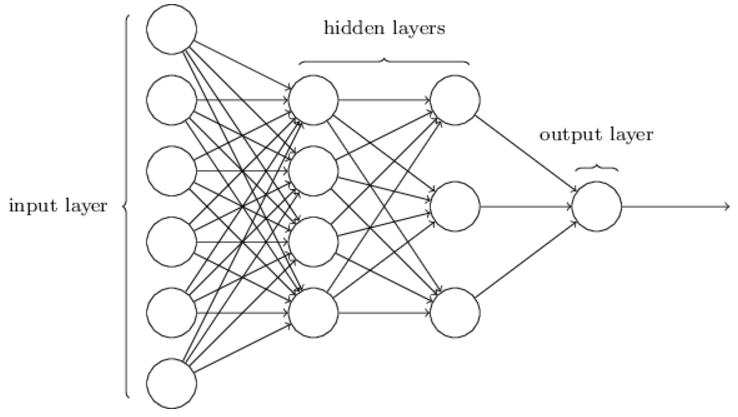
\includegraphics[scale=0.6]{Bilder/neural_network_extended}
	\caption{Aufbau des neuronalen Netzwerks hinsichtlich der einzelnen Layer.} 
	\label{fig:neural_network_extended} 
\end{figure}

\noindent
Für die Zusammensetzung von Eingabe- und Ausgabeschichten in einem Netzwerk, fällt die Betrachtung auf die Erkennung einer handgeschrieben "9". Als Eingabewerte dienen dem Netzwerk die Intensitäten der Bildpixel. Liegt ein Graustufenbild der Größe von 64x64 Pixeln vor, leiten sich daraus 4096 Eingabeknoten  mit skalierten Intensitätswerten zwischen 0 und 1 ab. Die Ausgabeschicht beinhaltet dagegen nur ein Neuron, um eine entsprechende Klassifizierung der "9" vornehmen zu können. \\[0.2cm]
\hspace*{1.3cm}
$ 
\begin{array}[t]{lcll}
	\mathtt{output} < 0.5 \quad\rightarrow\quad \mbox{"Eingabebild ist keine 9"} \\[0.2cm]
	\mathtt{output} \geq 0.5 \quad\rightarrow\quad \mbox{"Eingabebild ist eine 9"}
\end{array}
$
\\[0.2cm]
Im Vergleich hierzu ist der Aufbau der Hidden-Layer nicht durch irgendwelche Regeln ableitbar. Zum Einsatz kommen Heuristiken, die das Verhalten eines Netzwerkes bestimmen, welches ausgehend vom Experiment erwartet und gewünscht wird. Zum Beispiel kann Untersucht werden, wie die Lernrate des Netzwerks sich im Verhältnis zu der Anzahl an Hidden-Layer verhält. \\

\noindent
Bisher viel die Betrachtung in dieser Arbeit auf neuronale Netze, bei denen die Ausgabe einer Schicht die Eingabe in der nächsten Schicht darstellte. Solche Netzwerke werden auch \textit{Feedforward Neural Networks} bezeichnet. Hierunter ist das das nicht Auftreten von Schleifen zu verstehen - sprich, Informationen werden im Netzwerk immer von Layer $n$ zu Layer $n+1$ übergeben. Somit kann verhindert werden, dass das Netzwerk in gewissen Fällen bei der Eingabe der Sigmoid-Funktion $\sigma$ von dessen Ausgabe abhängig ist. \\
Ebenfalls gibt es Netzwerke bei denen sogenannte \textit{Feedback Loops} möglich sind. In diesem Fall handelt es sich um \textit{Recurrent Neural Networks}. Die Idee hinter diesem Modell ist, dass bestimmte Neuronen über einen definierten Zeitraum aktiv sind bevor sie inaktiv werden. Dies kann andere Neuronen anregen, ebenfalls über einen gewissen Zeitraum aktiv zu sein und eine entsprechende Kettenreaktion auslösen (Kaskade). Schleifen stellen in diesem Modell kein Problem dar, da die Ausgabe eines Neurons erst zu einem späteren Zeitpunkt die Eingabe beeinflusst. \\
Stellt man diese Arten von neuronalen Netzwerken gegenüber, so lässt sie zum heutigen Zeitpunkt die Aussage treffen, dass Feedback Neural Networks weniger Verbreitung finden. Dies ist begründet in der Leistungsfähigkeit der Lernalgorithmen. Jedoch sollte an dieser Stelle berücksichtigt werden, dass mittels Feedback Neural Networks bestimmte Probleme mit einem geringeren architektonischen Aufwand gelöst werden können. Darüber hinaus bildet der komplexere logische Aufbau eines solchen Netzwerks, das menschliche Verhalten besser ab.

\section{Perceptrons}
Ein Perceptron ist ein mathematisches Modell zur Abbildung eines künstliches Neurons in einem Netzwerk. Es wird für die Entscheidungsfindung herangezogen, indem verschiedene Aussagen abgewägt werden. Hierbei nimmt das Perceptron eine Menge von Eingaben $x_n$ mit $n \in \{1, \cdots, m\}$ und berechnet einen einzigen binären Ausgabewert (siehe Abb. \ref{fig:perceptron}). 
\begin{figure}[hbt]
	\centering
	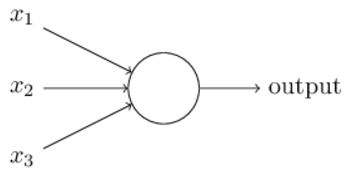
\includegraphics[scale=0.6]{Bilder/perceptron}
	\caption{Percetron mit den Eingaben $x_1, x_2, x_3$ und der Ausgabe $\mathtt{output}$.} 
	\label{fig:perceptron} 
\end{figure}

\noindent
Für jeden Eingabewert $x_n$ wird eine Gewichtung $w_n$ mit $n \in \{1, \cdots, m\}$ zugeordnet. Der Ausgabewerte $\mathtt{output}$ wird mittels der gewichteten Summe $\sum_j w_j x_k$ und einem definierten Grenzwert $\mathtt{threshold}$ bestimmt.
\begin{equation}
	\mathtt{output} := \left\{
	\begin{array}{ll}
 		0 & \displaystyle \mbox{falls}\quad \sum\limits_j w_j x_j \leq \mathtt{threshold} \\[0.5cm]
 		1 & \displaystyle \mbox{falls}\quad \sum\limits_j w_j x_j > \mathtt{threshold}
	\end{array}\right.
\end{equation}

\noindent
Der Aufbau des Netzwerks leitet sich aus den unterschiedlichen Modellen der Entscheidungsfindung ab und wird mit Hilfe der Perceptrons abgebildet (siehe Abb. \ref{fig:perceptron_models}).
\begin{figure}[hbt]
	\centering
	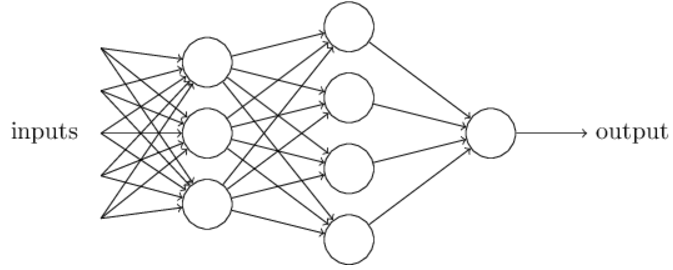
\includegraphics[scale=0.75]{Bilder/perceptron_models}
	\caption{Unterschiedliche Möglichkeiten der Entscheidungsfindung.} 
	\label{fig:perceptron_models} 
\end{figure}
Eine Entscheidungsmöglichkeit wird hierbei durch das Perceptron dargestellt. Weiterhin wird eine Spalte von Perceptrons als \textit{Layer} bezeichnet. Der erste Layer fällt Entscheidungen auf Basis der Eingabewerte, indem er diese abwägt. Jedes Perceptron des zweiten Layers hingegen, wägt für die Entscheidungsfindung die Resultate des ersten Layers ab. Ein Perceptron auf dem zweiten Layer kann somit eine Entscheidung auf einer abstrakteren und komplexeren Ebene durchführen. Auf diese Weise kann sich ein vielschichtiges Netzwerk von Perceptrons in ein anspruchsvolles Modell zur Entscheidungsfindung entwickeln. \\

\noindent
Im folgenden wird die mathematische Beschreibung von Perceptrons vereinfacht, indem Änderungen an der Notation für $\sum_j w_j x_j > \mathtt{threshold}$ vorgenommen werden. Für die Beschreibung der Summe $\sum_j w_j x_j$ werden die Vektoren $\mathbf{w}$ und $\mathbf{x}$ eingeführt, wodurch sich die Schreibweise $\mathbf{w} \cdot \mathbf{x} \equiv \sum_j w_j x_j$ ergibt. Des Weiteren wird der $\mathtt{threshold}$ auf die andere Seite der Ungleichung gezogen und erhält die Bezeichnung \textit{Bias}, $b \equiv \mathtt{-threshold}$. 
\begin{equation}
	\mathtt{output} := \left\{
	\begin{array}{ll}
 		0 & \displaystyle \mbox{falls}\quad \mathbf{w} \cdot \mathbf{x} + b \leq 0 \\[0.2cm]
 		1 & \displaystyle \mbox{falls}\quad \mathbf{w} \cdot \mathbf{x} + b > 0
	\end{array}\right.
\end{equation}

\noindent
Dieses mathematische Verhalten wird durch die folgende Stufenfunktion verdeutlicht (Abb. \ref{fig:perceptron_plot}).
\begin{figure}[hbt]
	\centering
	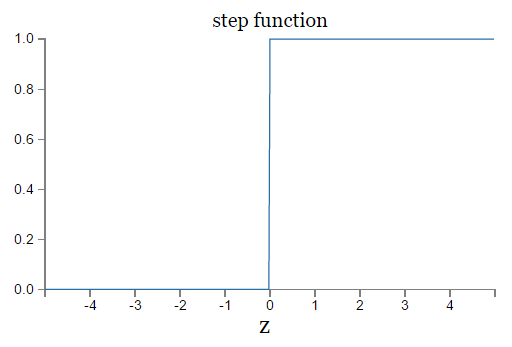
\includegraphics[scale=0.6]{Bilder/perceptron_plot}
	\caption{Sigmoid Funktion $\sigma(z)$.} 
	\label{fig:perceptron_plot} 
\end{figure}

\section{Sigmoid Neurons}
Für die Entwicklung lernender Algorithmen in einem Netzwerk mit Perceptrons, fällt unsere Betrachtung auf das Beispiel der Erkennung von handgeschriebenen Zahlen. Die Eingabe für das Netzwerk könnten die Raw Pixeldaten der eingescannten Bilder darstellen, welche die handgeschriebenen Zahlen abbilden. Das Ziel an dieser Stelle ist, dass das Netzwerk anhand der Veränderungen von \textit{Weights} und \textit{Biases} lernt eine korrekte Klassifizierung der Zahlen vorzunehmen. \\
Das Modifizieren der \textit{Weights} und \textit{Biases} kann das Verhalten des Netzwerkes und deren Entscheidungsfindung zu Problemen beeinflussen. Angenommen die Erkennung und Klassifizierung einer Zahl wurde durch das Netzwerk falsch vorgenommen, so können durch kleine Veränderungen an den \textit{Weights} und \textit{Biases} eine Korrektur durchgeführt werden. Dieses stetige Modifizieren der Werte über einen definierten Zeitraum ermöglicht ein lernendes Netzwerk (siehe Abb. \ref{fig:sigmoid_learning}). 
\begin{figure}[hbt]
	\centering
	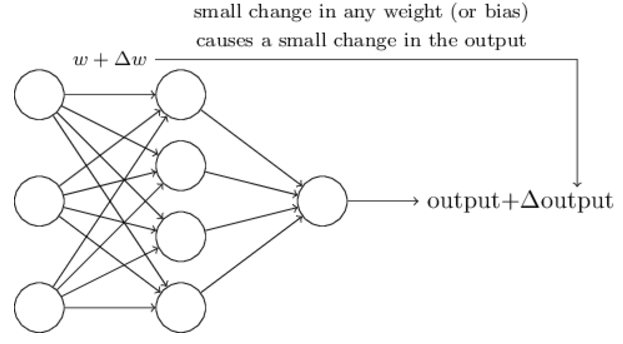
\includegraphics[scale=0.7]{Bilder/sigmoid_learning}
	\caption{Modifizieren von Weights und Biases schaffen lernendes Netzwerk.} 
	\label{fig:sigmoid_learning} 
\end{figure}

\noindent
Dieses wünschenswerte Verhalten eines lernenden Netzwerks kann durch Perceptrons nicht gewährleistet werden, da eine Veränderung der Weights und Biases den Ausgabewerte $\mathtt{output}$ eines Neurons umkehren kann. Dadurch kann das komplette Verhalten zur Klassifizierung von Zahlen beeinflusst werden, wobei zuvor falsch erkannte Zahlen nun richtig klassifiziert werden und umgekehrt. Mit Hilfe der Einführung des Sigmoid Neurons soll dieser Fehler behoben werden. Eine Änderung der Weights und Biases bei diesem künstlichen Neuron soll nur marginale Änderungen an dem Ausgabewert $\mathtt{output}$ vornehmen. Diese Erweiterung des Neurons begünstigt ein Netzwerk selbständig die Klassifizierung von Zahlen zu optimieren. \\

\noindent
Der Aufbau des Sigmoid Neurons ähnelt dem Perceptron, wobei das Neuron eine Anzahl von Eingabewerten $x_n$ mit $n \in \{1, \cdots ,m\}$ entgegennimmt und ausgehend von diesen Informationen den $\mathtt{output}$ ermittelt. Der wesentliche Unterschied zwischen diesen zwei Typen von Neuronen liegt in dem Wertebereich des $\mathtt{output}$. Bei dem Sigmoid Neuron kann dieser alle Werte zwischen 0 und 1 annehmen, sprich $\mathtt{output} \in [0 .. 1]$. Weiterhin weist auch diese Art von Neuronen für jeden Eingabewert eine Gewichtung $w_n$ mit $n \in \{1 .. n\}$ sowie einen Bias auf. \\
Für die Berechnung des $\mathtt{output}$ wird in diesem Kontext die \textit{Sigmoid Funktion} $\sigma(z)$ angewendet.
\begin{equation}
	\sigma(z) \equiv \frac{1}{1+e^{-z}} \quad\mbox{mit}\quad z = w \cdot x + b
\end{equation}
Unter Berücksichtigung der Eingabewerte $x_n$ mit $n \in \{1 .. n\}$ und der Weights  $w_n$ mit $n \in \{1 .. n\}$ ergibt sich die folgende Formel:
\begin{equation}
	\sigma(z) \equiv \frac{1}{1+\exp(-\sum_j w_j x_j - b)}
\end{equation}
Dabei weist das Sigmoid Neuron weiterhin das gleiche Verhalten wie ein Perceptron auf, wenn eine Grenzwertbetrachtung durchführt wird. \\[0.2cm]
\hspace*{1.3cm}
$
\begin{array}[t]{lcll}
	\lim\limits_{z \to \infty}{\sigma(z)} \approx 1 \quad\quad bzw. \\[0.2cm]
	\lim\limits_{z \to -\infty}{ \sigma(z)} \approx 0
\end{array}
$
\\[0.2cm]
Dieses Verhalten wird weiterhin verdeutlicht, wenn die Betrachtung auf den folgenden Funktionsgraph fällt (siehe Abb. \ref{fig:sigmoid_plot}). Für große $z$ nimmt die Funktion den Wert 1 an und für kleine $z$ nimmt die Funktion den Wert 0 an.
\begin{figure}[hbt]
	\centering
	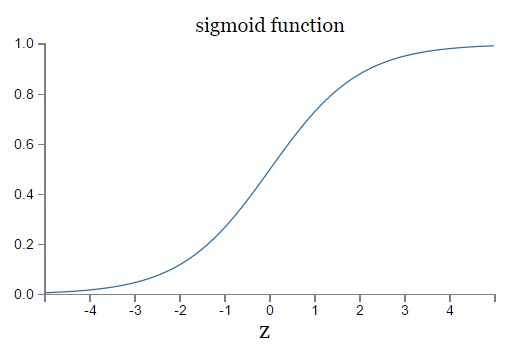
\includegraphics[scale=0.6]{Bilder/sigmoid_plot}
	\caption{Sigmoid Funktion $\sigma(z)$.} 
	\label{fig:sigmoid_plot} 
\end{figure}

\noindent
Im Vergleich hierzu die Stufenfunktion, die das Verhalten eines Perceptrons abbildet (siehe Abb. \ref{fig:perceptron_plot}).
\begin{figure}[hbt]
	\centering
	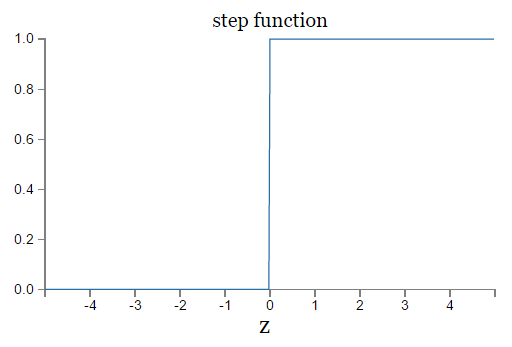
\includegraphics[scale=0.6]{Bilder/perceptron_plot}
	\caption{Sigmoid Funktion $\sigma(z)$.} 
	\label{fig:perceptron_plot} 
\end{figure}
Die Vorteile der Sigmoid Funktion liegen in den marginalen Änderungen $\delta w_j$ bei den Gewichtungen und $\delta b$ im Bias, welche eine marginale Änderung am $\delta\mathtt{output}$ vornehmen. Damit stellt $\delta\mathtt{output}$ die lineare Funktion bezüglich der Änderungen  $\delta w_j$ und $\delta b$ in den Weights und Bias dar.
\begin{equation}
	\Delta\mathtt{output} \equiv \sum_{j}{\frac{\partial\mathtt{output}}{\partial w_j}\Delta w_j+\frac{\partial\mathtt{output}}{\partial b}\Delta b_j}
\end{equation}
Diese Linearität begünstigt die Wahl von kleinen Änderungen in den Weights und Biases, um das Verhalten für ein lernendes Netzwerk abzuleiten.   

\section{Netzwerk zur Klassifizierung von handgeschrieben Zahlen}